% Section 3: Other Repeated Games
%-------------------------------------------------------------------------------

\begin{frame}{A More Complicated Game}
  \begin{center}
  \begin{tabular}{*{5}{c|}}
  	\multicolumn{2}{c}{} & \multicolumn{3}{c}{Player $j$}\\ \cline{3-5}
    \multicolumn{1}{c}{} &   & x & y & z \\\cline{2-5}
    \multirow{3}*{Player $i$}  & x & 5, 5 & 2, 7 & 1, 3 \\\cline{2-5}
                             & y & 7, 2 & 3, 3 & 0, 1 \\\cline{2-5}
                             & z & 3, 1 & 1, 0 & 2, 2 \\\cline{2-5}
  \end{tabular}
  \end{center}
  What are the \textbf{pure strategy Nash equilibria} of the \textit{one-shot} game?
\end{frame}

\begin{frame}{A More Complicated Game}
  \begin{center}
  \begin{tabular}{*{5}{c|}}
  	\multicolumn{2}{c}{} & \multicolumn{3}{c}{Player $j$}\\ \cline{3-5}
    \multicolumn{1}{c}{} &       & x    & y    & z    \\\cline{2-5}
    \multirow{3}*{Player $i$}  & x & 5, 5 & 2, \underline{7} & 1, 3 \\\cline{2-5}
                             & y & \underline{7}, 2 & \underline{3}, \underline{3} & 0, 1 \\\cline{2-5}
                             & z & 3, 1 & 1, 0 & \underline{2}, \underline{2} \\\cline{2-5}
  \end{tabular}
  \end{center}
  What are the \textbf{pure strategy Nash equilibria} of the \textit{one-shot} game?
  \begin{itemize}
    \pause
    \item (y,y) and (z,z)
    \pause
    \item Any other strategy profile is not \textit{stable} in the one-shot game
    \begin{itemize}
      \item for example, (x,x); either player would deviate to y
    \end{itemize}
  \end{itemize}
\end{frame}

\begin{frame}{Repeated Game with 3 strategies per period}
  Now suppose that this game is played repeatedly an infinite number of times.  
  \begin{center}
  \begin{tabular}{*{5}{c|}}
  	\multicolumn{2}{c}{} & \multicolumn{3}{c}{Player $j$}\\ \cline{3-5}
    \multicolumn{1}{c}{} &       & x    & y    & z    \\\cline{2-5}
    \multirow{3}*{Player $i$}  & x & 5, 5 & 2, \underline{7} & 1, 3 \\\cline{2-5}
                             & y & \underline{7}, 2 & \underline{3}, \underline{3} & 0, 1 \\\cline{2-5}
                             & z & 3, 1 & 1, 0 & \underline{2}, \underline{2} \\\cline{2-5}
  \end{tabular}
  \end{center}
  \begin{itemize}
    \item Can we do better than the single period equilibrium? 
    \item Are there any \textit{Pareto improvements} to be made?
  \end{itemize}
\end{frame}

\begin{frame}{Grim Trigger}
  \underline{Player $i$} 
  \begin{align*}
    \begin{cases}
      t = 1 & \text{Play } x  \\ 
      t > 1 & 
      \begin{cases}
        \text{Play } x \text{ only if } s_j^1\dots s_j^{t-1} = x\\
        \text{Play } y \text{ if anything other than } x \text{ has been played} \\
      \end{cases}
    \end{cases} 
  \end{align*}

  \underline{Player $j$}
  \begin{itemize}
    \item $EV_{Coop} = \frac{5}{1-\delta}$ 
    \item $EV_{Cheat} = 7 + \frac{3\delta}{1-\delta}$
  \end{itemize}
\end{frame}

\begin{frame}{Grim Trigger}
  Solve for the value of $\delta$ for which this is a \textbf{SPNE}
  \pause
  \begin{align*}
    \frac{5}{1-\delta} & \geq 7 + \frac{3\delta}{1-\delta} \\
    5 + \frac{5\delta}{1-\delta} & \geq 7 + \frac{3\delta}{1-\delta} \\
    \frac{(5-3)\delta}{1-\delta} & \geq 7-5 \\
    \delta & \geq \frac{1}{2}
  \end{align*}
\end{frame}

\begin{frame}{Grim Trigger with harsher punishment}
  \begin{center}
  \begin{tabular}{*{5}{c|}}
  	\multicolumn{2}{c}{} & \multicolumn{3}{c}{Player $j$}\\ \cline{3-5}
    \multicolumn{1}{c}{} &       & x    & y    & z    \\\cline{2-5}
    \multirow{3}*{Player $i$}  & x & 5, 5 & 2, \underline{7} & 1, 3 \\\cline{2-5}
                             & y & \underline{7}, 2 & \underline{3}, \underline{3} & 0, 1 \\\cline{2-5}
                             & z & 3, 1 & 1, 0 & \underline{2}, \underline{2} \\\cline{2-5}
  \end{tabular}
  \end{center}
  The fallback strategy $y$ is not the harshest punishment.
  \begin{itemize}
    \item $z$ is still \textit{credible} 
    because it is another NE of the stage game
  \end{itemize}
\end{frame}

\begin{frame}{Grim Trigger with harsher punishment}
  With $z$ as the fallback punishment strategy:
  \begin{align*}
    \begin{cases}
      t = 1 & \text{Play } x  \\ 
      t > 1 & 
      \begin{cases}
        \text{Play } x \text{ if only } x \text{ has been played previously} \\
        \text{Play } \textbf{z} \text{ if anything other than } x \text{has been played} \\
      \end{cases}
    \end{cases} 
  \end{align*}
    \begin{align*}
      EU_{\text{Coop}} = 5 + 5\delta + 5\delta^2 \dots & 
      = 5 + \frac{5\delta}{1-\delta} \\
      EU_{\text{Cheat}} = 7 + \textbf{2} \delta + 2\delta^2 + \dots & 
      = 7 + \frac{2\delta}{1-\delta}
    \end{align*}
\end{frame}

\begin{frame}
  \begin{figure}[h]
    \centering
    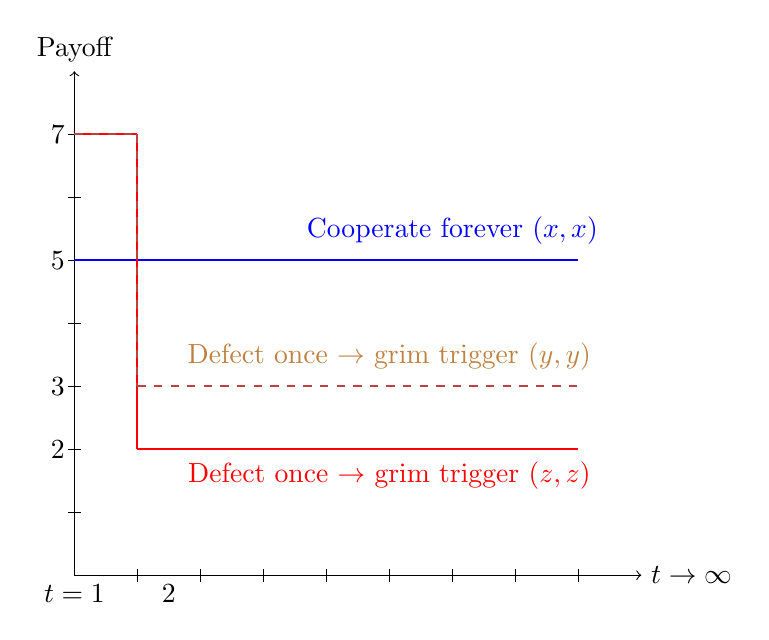
\begin{tikzpicture}[scale=0.8]
    % Axes
    \draw[->] (0,0) -- (9,0) node[right] {$t\rightarrow\infty$};
    \draw[->] (0,0) -- (0,8) node[above] {Payoff};
    % Ticks
    \foreach \x in {1,2,3,4,5,6,7,8}
      \draw (\x,0.1) -- (\x,-0.1);
    \foreach \y in {1,2,3,4,5,6,7}
      \draw (0.1,\y) -- (-0.1,\y);
    % Labels
    \node[left] at (0,5) {$5$};
    \node[left] at (0,2) {$2$};
    \node[left] at (0,3) {$3$};
    \node[left] at (0,7) {$7$};
    % --- Cooperate forever: constant at 5 ---
    \draw[thick, blue] (0,5) -- (8,5);
    \node[blue, above] at (6,5.1) {Cooperate forever $(x,x)$};
    % --- Defect once then harsh punishment z: 7 then 2 ---
    \draw[thick, red] (0,7) -- (1,7);
    \draw[thick, red] (1,7) -- (1,2);
    \draw[thick, red] (1,2) -- (8,2);
    \node[red, above] at (5,1.2) {Defect once $\rightarrow$ grim trigger $(z,z)$};
    % --- Defect once then soft punishment y: 7 then 3 ---
    \draw[thick, dashed, red!50!gray] (0,7) -- (1,7);
    \draw[thick, dashed, red!50!gray] (1,7) -- (1,3);
    \draw[thick, dashed, red!50!gray] (1,3) -- (8,3);
    \node[orange!50!gray, above] at (5,3.1) {Defect once $\rightarrow$ grim trigger $(y,y)$};
    % Period labels
    \node[below] at (0,0) {$t=1$};
    \node[below] at (1.5,0) {2};
    \end{tikzpicture}
    % \caption{Payoff paths under cooperation and grim-trigger punishments at $(z,z)$ and $(y,y)$}
    \end{figure}
\end{frame}

\begin{frame}{Grim Trigger with harsher punishment}
  Harsher punishments make cooperation easier to sustain:
  \begin{align*}
    \frac{5}{1-\delta} & \geq 7 + \frac{2\delta}{1-\delta} \\
    5 + \frac{5\delta}{1-\delta} & \geq 7 + \frac{2\delta}{1-\delta} \\
    \frac{(5-2)\delta}{1-\delta} & \geq 7-5 \\
    \delta & \geq \frac{2}{5}
  \end{align*}
\end{frame}

\begin{frame}{Tit-for-Tat}
  \underline{Player $i$} 
  \begin{align*}
    \begin{cases}
      t = 0 & \text{Play } x  \\ 
      t > 0 & \text{Play Player $j$'s strategy from } t-1 \\
    \end{cases} 
  \end{align*}

  \underline{Player $j$}
  \begin{itemize}
    \item In period $t=1$, cheat by playing $y$ to get payoff of 7
    \item In period $t>1$, go back to playing cooperatively
    \item $EV_{\text{Coop}} = 5 + 5\delta + \dots \frac{5}{1-\delta}$ 
    \item $EV_{\text{Cheat once}} = 7 + 2\delta + 5\delta^2 + 5\delta^3 + \dots = 7 + 2\delta + \frac{5\delta^2}{1-\delta}$
  \end{itemize}
\end{frame}

\begin{frame}{Tit-for-Tat}
  Solve for the value of $\delta$ for which this is a \textbf{SPNE}
  \begin{align*}
    5 + 5\delta + \frac{5\delta^2}{1-\delta} \geq & 7 + 2\delta + \frac{5\delta^2}{1-\delta} \\
    5 + 5\delta & \geq 7 + 2\delta \\
    \delta & \geq \frac{2}{3}
  \end{align*}
\end{frame}

\begin{frame}
  \begin{figure}[h]
    \centering
    \begin{tikzpicture}[scale=0.8]
    % Axes
    \draw[->] (0,0) -- (9,0) node[right] {$t\rightarrow\infty$};
    \draw[->] (0,0) -- (0,8) node[above] {Payoff};
    % Ticks
    \foreach \x in {1,2,3,4,5,6,7,8,9}
      \draw (\x,0.1) -- (\x,-0.1);
    \foreach \y in {1,2,3,4,5,6,7,8}
      \draw (0.1,\y) -- (-0.1,\y);
    % Labels
    \node[left] at (0,5) {$5$};
    \node[left] at (0,2) {$2$};
    \node[left] at (0,7) {$7$};
    % --- Cooperate forever: constant at 5 ---
    \draw[thick, blue] (0,5) -- (9,5);
    \node[blue, above] at (6,5.2) {Cooperate forever $(x,x)$};
    % --- Deviate once to y, then punished by z for one period, then forgiven ---
    \draw[thick, red] (0,7) -- (1,7);        % t=1 payoff = 7
    \draw[thick, red] (1,7) -- (1,3);        % drop to punishment
    \draw[thick, red] (1,3) -- (2,3);        % t=2 payoff = 3
    \draw[thick, red] (2,3) -- (2,5);        % forgiveness jump
    \draw[thick, red] (2,5) -- (9,5);        % back to cooperation
    \node[red, above] at (6,4.2) {Cheat once $y$ $\rightarrow$ TFT forgiveness};
    % Period labels
    \node[below] at (0,0) {$t=1$};
    \node[below] at (1.5,0) {2};
    \node[below] at (2.5,0) {3};
    \end{tikzpicture}
    % \caption{Payoff paths under cooperation and one-period-forgiveness Tit-for-Tat}
    \end{figure}
\end{frame}

\begin{frame}{A reciprocating cooperation strategy}
    \underline{Player $i$}
    $
      \begin{cases}
        t=0 & \text{Play } y \\ 
        t>0 & 
        \begin{cases}
          \text{Play } y \text{ if } t \text { is even } \\ 
          \text{Play } x \text{ if } t \text { is odd } \\ 
          \text{Play } z \text{ forever } 
          \text{ if P2 played } y 
          \text{ when $t$ is even} \\ 
        \end{cases}
      \end{cases} 
    $

    \underline{Player $j$}
    $
      \begin{cases}
        t=0 & \text{Play } x \\ 
        t>0 & 
        \begin{cases}
          \text{Play } y \text{ if } t \text { is odd } \\ 
          \text{Play } x \text{ if } t \text { is even } \\ 
          \text{Play } z \text{ forever } 
          \text{ if P2 played } y 
          \text{ when $t$ is odd} \\ 
        \end{cases}
      \end{cases} 
      $
\end{frame}

\begin{frame}{SPNE with reciprocation}
  What if Player $j$ defects in period 1?
  \begin{itemize}
    \item $EV_2(\text{Defect}) = 3 + 2\delta + 2\delta^2 + \dots = 3 + \frac{2\delta}{1-\delta}$
    \item $EV_2(\text{Coop}) = 2 + 7\delta + 2 \delta^2 + \dots = \frac{2+7\delta}{1-\delta^2}$
  \end{itemize}
  \begin{align*}
    \frac{2+7\delta}{1-\delta^2} & \geq 3 + \frac{2\delta}{1-\delta} \\
    \dots & \dots \\
    \delta^2 + 5\delta - 1 & \geq 0 \\
    \delta & > \approx 0.65 \\
  \end{align*}
\end{frame}

\begin{frame}{When can cooperation be achieved?}
  With all of these different ways of achieving repeated cooperation, 
  you might be wondering if there is a way to tell what strategies can actually work
  \begin{itemize}
    \item Punishment outcome must be BR in stage game
    \item Punishment strategies can't be exploitable (only credible threats)
    \item Different coordinating strategies are sustainable for different discount factors
  \end{itemize}
\end{frame}

\begin{frame}{Folk Theorem}
  Any strategy is a potential SPNE for a \textbf{repeated} stage game if: 
  \begin{itemize}
    \item Both agents are sufficiently patient and far-sighted (high enough $\delta$)
    \item The payoffs from the cooperative strategy profile satisfy the two properties: 
    \begin{itemize}
      \item \textbf{Individually Rational:} the payoffs to each agent (weakly) exceed their minimax payoffs in the stage game 
      \item \textbf{Feasibility:} the payoffs are weighted averages of the payoffs found in the stage game
    \end{itemize}
  \end{itemize}
\end{frame}

\begin{frame}{Folk Theorem with 3x3 Repeated Game Example}
  \begin{center}
  \begin{tabular}{*{5}{c|}}
  	\multicolumn{2}{c}{} & \multicolumn{3}{c}{Player $j$}\\ \cline{3-5}
    \multicolumn{1}{c}{} &       & x    & y    & z    \\\cline{2-5}
    \multirow{3}*{Player $i$}  & x & 5, 5 & 2, \underline{7} & 1, 3 \\\cline{2-5}
                             & y & \underline{7}, 2 & \underline{3}, \underline{3} & 0, 1 \\\cline{2-5}
                             & z & 3, 1 & 1, 0 & \underline{2}, \underline{2} \\\cline{2-5}
  \end{tabular}
  \end{center}
  The \alert{Minimax} equilibrium is (z,z)
  \begin{itemize}
    \item it \textit{minimizes} the \textit{maximum} payoff that your opponent could get
    \item The Minimax payoffs in this stage game are (2, 2)
    \item Intuitively, this is the \textit{safe} option: you can always fall back on it if cooperation fails
  \end{itemize}
\end{frame}

\begin{frame}{Incentive Compatible and Individually Rational conditions in 3x3 repeated game}
  \begin{figure}[!h]
  \centering
  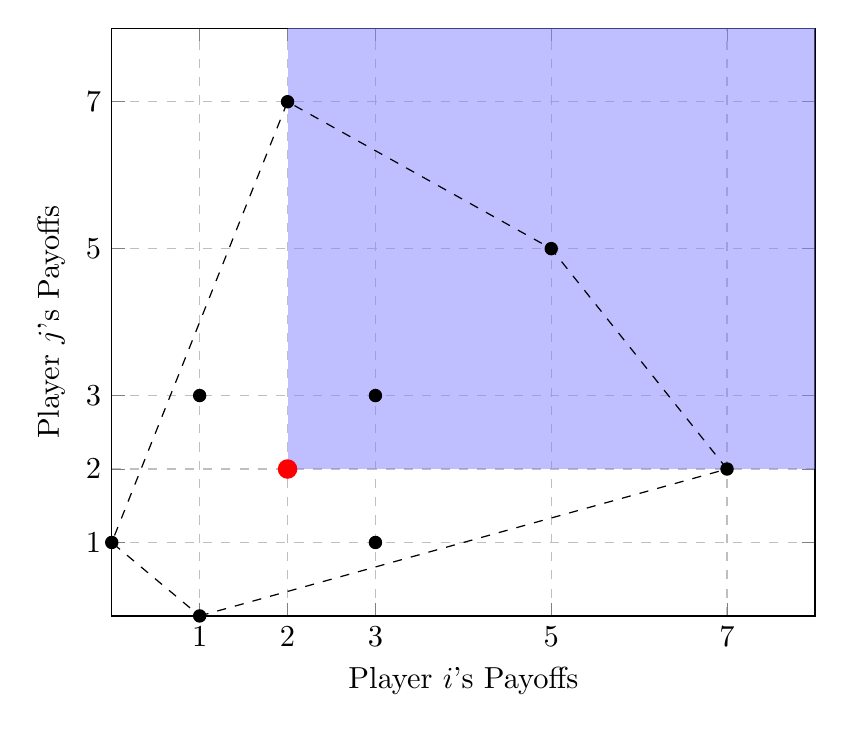
\begin{tikzpicture}[scale=1.1]
  \begin{axis}[
    width=0.8\textwidth,
    grid,
    xlabel={Player $i$'s Payoffs},
    ylabel={Player $j$'s Payoffs},
    xmin=0, xmax=8,
    ymin=0, ymax=8,
    xtick={1,2,3,5,7},
    ytick={1,2,3,5,7},
    grid style=dashed,
    legend style={at={(0.03,0.97)},anchor=north west},
  ]
  % --- Shaded Pareto-dominant region relative to (2,2) ---
  \addplot[
    fill=blue!50,
    fill opacity=0.5,
    draw=none
  ] coordinates {
    (2,2)
    (8,2)
    (8,8)
    (2,8)
  } -- cycle;
  % \addlegendentry{Pareto-dominates $(2,2)$}
  % --- Outline of the convex hull
  \addplot[
    dashed
  ] coordinates{
    (1,0)
    (7,2)
    (5,5)
    (2,7)
    (0,1)
  } --cycle;
  % --- Plot all payoff points ---
  \addplot[only marks]
  coordinates {
  (5,5) (2,7) (1,3) 
  (7,2) (3,3) (0,1)
  (3,1) (1,0) (2,2)
  };
  % \addlegendentry{Stage-game payoffs}
  % --- Highlight the minimax point (2,2) ---
  \addplot[
    only marks,
    mark=*,
    mark size=3,
    color=red
  ] coordinates {(2,2)};
  % \addlegendentry{Minimax $(2,2)$}
  \end{axis}
  \end{tikzpicture}
\end{figure}
\end{frame}

\begin{frame}{Folk Theorem with 3x3 Repeated Game Example}
  \begin{itemize}
    \item The shaded region of the graph shows us all of the strategy profiles which could be sustained by the \textbf{Folk Theorem} 
    \item This shows us why that strategy profile of alternating between (x, y) and (y, x) worked: 
    \begin{itemize}
      \item even though getting 2 on even or odd periods was no better than the Minimax payoffs, because you could alternate with the higher payoff of 7 you could do better as long as you are patient enough 
      \item this mix between (2, 7) and (7, 2) is \textit{within the convex hull} of feasible payoffs
    \end{itemize}
  \end{itemize} 
\end{frame}

% \begin{frame}{Cooperation in Repeated Games}
%   \begin{itemize}
%     \item As you can probably tell, there are an infinite number of strategy profiles which can achieve cooperation 
%     \begin{itemize}
%       \item We could allow for mixed strategies, which would work similar to the alternating example we saw 
%       \item The Folk Theorem tells us that all we need is for all players to be patient enough 
%       \item and also that the past plays are common knowledge
%     \end{itemize}
%   \end{itemize}
% \end{frame}

\begin{frame}{Importance of the Folk Theorem}
  Why does this matter for real life? 
  \begin{itemize}
    \item Most strategic interactions in your life are repeated 
    \item Even when you don't repeatedly interact with the same exact people, you still see cooperative outcomes 
    \item \textbf{Institutions, Reputations, and Social Structures} all serve to allow for past interactions to be common knowledge
    \item The history of humanity is built on how we arrange our strategic interactions in ways so that people are incentivized to play nice with others
  \end{itemize}
\end{frame}

\begin{frame}{Importance of the Folk Theorem}
  Some caveats:
  \begin{itemize}
    \item People can't know exactly when the game will end
    \begin{itemize}
      \item Institutions have to \textit{seem} like they are infinitely lived (compared to finitely lived humans)
    \end{itemize}
    \item Cooperative equilibria must beat outside options 
    \begin{itemize}
      \item If you make your institution too costly for people to engage with, they will opt out 
    \end{itemize}
    \item People need to be patient enough 
    \item Punishments must be credible
  \end{itemize}
\end{frame}
